%Version 3 December 2023
% See section 11 of the User Manual for version history
%
%%%%%%%%%%%%%%%%%%%%%%%%%%%%%%%%%%%%%%%%%%%%%%%%%%%%%%%%%%%%%%%%%%%%%%
%%                                                                 %%
%% Please do not use \input{...} to include other tex files.       %%
%% Submit your LaTeX manuscript as one .tex document.              %%
%%                                                                 %%
%% All additional figures and files should be attached             %%
%% separately and not embedded in the \TeX\ document itself.       %%
%%                                                                 %%
%%%%%%%%%%%%%%%%%%%%%%%%%%%%%%%%%%%%%%%%%%%%%%%%%%%%%%%%%%%%%%%%%%%%%

%%\documentclass[referee,sn-basic]{sn-jnl}% referee option is meant for double line spacing

%%=======================================================%%
%% to print line numbers in the margin use lineno option %%
%%=======================================================%%

%%\documentclass[lineno,sn-basic]{sn-jnl}% Basic Springer Nature Reference Style/Chemistry Reference Style

%%======================================================%%
%% to compile with pdflatex/xelatex use pdflatex option %%
%%======================================================%%

%%\documentclass[pdflatex,sn-basic]{sn-jnl}% Basic Springer Nature Reference Style/Chemistry Reference Style


%%Note: the following reference styles support Namedate and Numbered referencing. By default the style follows the most common style. To switch between the options you can add or remove “Numbered” in the optional parenthesis. 
%%The option is available for: sn-basic.bst, sn-vancouver.bst, sn-chicago.bst%  
 
%%\documentclass[pdflatex,sn-nature]{sn-jnl}% Style for submissions to Nature Portfolio journals
%%\documentclass[pdflatex,sn-basic]{sn-jnl}% Basic Springer Nature Reference Style/Chemistry Reference Style
\documentclass[pdflatex,sn-mathphys-num]{sn-jnl}% Math and Physical Sciences Numbered Reference Style 
%%\documentclass[pdflatex,sn-mathphys-ay]{sn-jnl}% Math and Physical Sciences Author Year Reference Style
%%\documentclass[pdflatex,sn-aps]{sn-jnl}% American Physical Society (APS) Reference Style
%%\documentclass[pdflatex,sn-vancouver,Numbered]{sn-jnl}% Vancouver Reference Style
%%\documentclass[pdflatex,sn-apa]{sn-jnl}% APA Reference Style 
%%\documentclass[pdflatex,sn-chicago]{sn-jnl}% Chicago-based Humanities Reference Style

%%%% Standard Packages
%%<additional latex packages if required can be included here>

\usepackage{graphicx}%
\usepackage{multirow}%
\usepackage{amsmath,amssymb,amsfonts}%
\usepackage{amsthm}%
\usepackage{mathrsfs}%
\usepackage[title]{appendix}%
\usepackage{xcolor}%
\usepackage{textcomp}%
\usepackage{manyfoot}%
\usepackage{nameref}%
\usepackage{booktabs}%
\usepackage{algorithm}%
\usepackage{algorithmicx}%
\usepackage{algpseudocode}%
\usepackage{listings}%

\usepackage{xr}
% \makeatletter
% \newcommand*{\addFileDependency}[1]{% argument=file name and extension
%   \typeout{(#1)}
%   \@addtofilelist{#1}
%   \IfFileExists{#1}{}{\typeout{No file #1.}}
% }
% \makeatother

% \newcommand*{\myexternaldocument}[1]{%
%     \externaldocument{#1}%
%     \addFileDependency{#1.tex}%
%     \addFileDependency{#1.aux}%
% }
% \myexternaldocument{si}

\externaldocument{si}

\makeatletter
\@input{xx.tex}
\makeatother

\definecolor{codegreen}{rgb}{0,0.6,0}
\definecolor{codegray}{rgb}{0.5,0.5,0.5}
\definecolor{codepurple}{rgb}{0.58,0,0.82}
\definecolor{backcolour}{rgb}{0.95,0.95,0.92}

\lstdefinestyle{mystyle}{
    backgroundcolor=\color{backcolour},   
    commentstyle=\color{codegreen},
    keywordstyle=\color{magenta},
    numberstyle=\tiny\color{codegray},
    stringstyle=\color{codepurple},
    basicstyle=\ttfamily\footnotesize,
    breakatwhitespace=false,         
    breaklines=true,                 
    captionpos=b,                    
    keepspaces=true,                 
    numbers=left,                    
    numbersep=5pt,                  
    showspaces=false,                
    showstringspaces=false,
    showtabs=false,                  
    tabsize=2
}

\lstset{style=mystyle}
%%%%

%%%%%=============================================================================%%%%
%%%%  Remarks: This template is provided to aid authors with the preparation
%%%%  of original research articles intended for submission to journals published 
%%%%  by Springer Nature. The guidance has been prepared in partnership with 
%%%%  production teams to conform to Springer Nature technical requirements. 
%%%%  Editorial and presentation requirements differ among journal portfolios and 
%%%%  research disciplines. You may find sections in this template are irrelevant 
%%%%  to your work and are empowered to omit any such section if allowed by the 
%%%%  journal you intend to submit to. The submission guidelines and policies 
%%%%  of the journal take precedence. A detailed User Manual is available in the 
%%%%  template package for technical guidance.
%%%%%=============================================================================%%%%

%% as per the requirement new theorem styles can be included as shown below
\theoremstyle{thmstyleone}%
\newtheorem{theorem}{Theorem}%  meant for continuous numbers
%%\newtheorem{theorem}{Theorem}[section]% meant for sectionwise numbers
%% optional argument [theorem] produces theorem numbering sequence instead of independent numbers for Proposition
\newtheorem{proposition}[theorem]{Proposition}% 
%%\newtheorem{proposition}{Proposition}% to get separate numbers for theorem and proposition etc.

\theoremstyle{thmstyletwo}%
\newtheorem{example}{Example}%
\newtheorem{remark}{Remark}%

\theoremstyle{thmstylethree}%
\newtheorem{definition}{Definition}%

\raggedbottom
%%\unnumbered% uncomment this for unnumbered level heads

\begin{document}

\title[Article Title]{ASKCOS: an open source software suite for synthesis planning}

%%=============================================================%%
%% GivenName	-> \fnm{Joergen W.}
%% Particle	-> \spfx{van der} -> surname prefix
%% FamilyName	-> \sur{Ploeg}
%% Suffix	-> \sfx{IV}
%% \author*[1,2]{\fnm{Joergen W.} \spfx{van der} \sur{Ploeg} 
%%  \sfx{IV}}\email{iauthor@gmail.com}
%%=============================================================%%

\author[1]{\fnm{Zhengkai} \sur{Tu}}\email{ztu@mit.edu}
\author[2]{\fnm{Sourabh J.} \sur{Choure}}\email{sjchoure@mit.edu}
\author[2]{\fnm{Mun Hong} \sur{Fong}}\email{fong410@mit.edu}
\author[2]{\fnm{Jihye} \sur{Roh}}\email{jroh99@mit.edu}
\author[3]{\fnm{Itai} \sur{Levin}}\email{itail@mit.edu}
\author[4]{\fnm{Kevin} \sur{Yu}}\email{kyu3@mit.edu}
\author[2]{\fnm{Joonyoung F.} \sur{Joung}}\email{jjoung@mit.edu}
\author[2]{\fnm{Nathan} \sur{Morgan}}\email{knathan@mit.edu}
\author[2]{\fnm{Shih-Cheng} \sur{Li}}\email{scli@mit.edu}
\author[2]{\fnm{Xiaoqi} \sur{Sun}}\email{xiaoqis@mit.edu}
\author[2]{\fnm{Huiqian} \sur{Lin}}\email{linhq@mit.edu}
\author[2]{\fnm{Mark} \sur{Murnin}}\email{murninm@mit.edu}
\author[2]{\fnm{Jordan P.} \sur{Liles}}\email{jliles24@mit.edu}
\author[5]{\fnm{Thomas J.} \sur{Struble}}\email{Thomas.Struble@bms.com}
\author[6]{\fnm{Michael E.} \sur{Fortunato}}\email{mike.fortunato@novartis.com}
\author{\fnm{Mengjie} \sur{Liu}\textsuperscript{2,}\footnote[2]{Current affiliation: AstraZeneca. Work done while at MIT.}}\email{mjliu@mit.edu}
\author[2]{\fnm{William H.} \sur{Green}}\email{whgreen@mit.edu}
\author[2]{\fnm{Klavs F.} \sur{Jensen}}\email{kfjensen@mit.edu}
\author*[1,2]{\fnm{Connor W.} \sur{Coley}}\email{ccoley@mit.edu}

\affil[1]{\orgdiv{Department of Electrical Engineering and Computer Science}, \orgname{Massachusetts Institute of Technology}, \orgaddress{\street{77 Massachusetts Ave}, \city{Cambridge}, \state{MA}, \postcode{02139}, \country{USA}}}

\affil[2]{\orgdiv{Department of Chemical Engineering}, \orgname{Massachusetts Institute of Technology}, \orgaddress{\street{77 Massachusetts Ave}, \city{Cambridge}, \state{MA}, \postcode{02139}, \country{USA}}}

\affil[3]{\orgdiv{Department of Biological Engineering}, \orgname{Massachusetts Institute of Technology}, \orgaddress{\street{77 Massachusetts Ave}, \city{Cambridge}, \state{MA}, \postcode{02139}, \country{USA}}}

\affil[4]{\orgdiv{Center for Computational Science and Engineering}, \orgname{Massachusetts Institute of Technology}, \orgaddress{\street{77 Massachusetts Ave}, \city{Cambridge}, \state{MA}, \postcode{02139}, \country{USA}}}

\affil[5]{\orgname{Bristol Myers Squibb}, \orgaddress{\street{250 Water Street, \city{Cambridge}, \state{MA}, \postcode{02141}, \country{USA}}}}

\affil[6]{\orgname{Novartis Institutes for BioMedical Research, Inc.}, \orgaddress{\street{250 Massachusetts Avenue}, \city{Cambridge}, \state{MA}, \postcode{02139}, \country{USA}}}

% Abstract – up to 150 words, unreferenced
\abstract{The advancement of machine learning and the availability of large-scale reaction datasets have accelerated the development of data-driven models for computer-aided synthesis planning (CASP) in the past decade. Here, we detail the newest version of ASKCOS, an open source software suite for synthesis planning that makes available several research advances in a freely available, practical tool. Four one-step retrosynthesis models form the basis of both interactive planning and automatic planning modes. Retrosynthetic planning is complemented by other modules for feasibility assessment and pathway evaluation, including reaction condition recommendation, reaction outcome prediction, and auxiliary capabilities such as solubility prediction and quantum mechanical descriptor prediction. ASKCOS has assisted hundreds of medicinal, synthetic, and process chemists in their day-to-day tasks, complementing expert decision making. It is our belief that CASP tools like ASKCOS are an important part of modern chemistry research, and that they offer ever-increasing utility and accessibility.}

\keywords{synthesis planning, open source software, data-driven predictive chemistry}

%%\pacs[JEL Classification]{D8, H51}

%%\pacs[MSC Classification]{35A01, 65L10, 65L12, 65L20, 65L70}

\maketitle

\section{Introduction}\label{introduction}

% CWC suggested P1: Overview of synthesis planning task, brief history, amenability to algorithmic approaches

Synthesis planning describes a broad category of approaches for selecting experimental pathways and procedures during target-oriented synthesis.  While planning a synthesis campaign may require significant chemistry expertise and benefits from the years of training that many experienced chemists undergo, the well-defined yet combinatorially complex nature of synthesis planning renders this task particularly amenable to algorithmic reasoning. Formally, computer-aided synthesis planning (CASP) integrates a variety of computational methodologies that assist chemists with different tasks in this process, including identifying viable synthetic routes through retrosynthetic analysis, recommending reaction conditions, and predicting reaction outcomes.

Since the 1960s, chemists have sought to encode the rules of organic synthesis into automated computational systems~\citep{corey_computer-assisted_1969,warr_short_2014}. Early CASP tools generally relied on expert-encoded reaction rules and heuristics for making suggestions. In particular, for one-step retrosynthetic analysis~\citep{corey_robert_1988}, expert systems such as LHASA~\citep{corey_computer-assisted_1972} and SECS~\citep{wipke_simulation_1978} made use of reaction templates that encode chemical reaction rules based on molecular pattern matching; AIPHOS~\citep{funatsu_computer-assisted_1988} and WODCA~\citep{gasteiger_wodca_1990} were among the first to combine retrosynthesis, reaction condition suggestion, and product prediction into an integrated system. More recent advancements include tools like Chematica (now Synthia)~\citep{grzybowski_chematica_2018}, which leverages modern computational capabilities alongside expert-curated rules and heuristics to propose transformations, generating synthetic pathways for complex molecules that have been successfully implemented in the laboratory~\citep{klucznik_efficient_2018,mikulak-klucznik_computational_2020}. 

% CWC suggested P2: Renewed interest with ML and data-driven approaches in recent years

With the development of machine learning and the availability of reaction datasets containing millions of entries, there has been renewed interest in CASP with data-driven approaches~\citep{tu_predictive_2023,schwaller_machine_2022}. Many data-driven models for one-step retrosynthesis have been developed with formulations based on reaction template prediction~\citep{dai_retrosynthesis_2019,chen_deep_2021} or retrieval~\citep{coley_computer-assisted_2017,xie_retrosynthesis_2023}, machine translation~\citep{tu_permutation_2022,tetko_state---art_2020,zhong_root-aligned_2022}, graph edit prediction~\citep{sacha_molecule_2021,somnath_learning_2021}, as well as other generative models~\citep{igashov_retrobridge_2023,gainski_retrogfn_2024}. These one-step predictors have been integrated with various tree-search algorithms to navigate through the network of hypothetical reactions to identify synthetic pathways in which all starting materials are accessible~\citep{heifets_construction_2012,segler_planning_2018,kishimoto_depth-first_2019,schwaller_predicting_2020,chen_retro_2020}. Machine learning models have also been applied to other elements of synthesis planning such as reaction condition recommendation~\citep{gao_using_2018,maser_multilabel_2021,kwon_generative_2022,qian_predictive_2023,chen_enhancing_2024} and reaction outcome prediction~\citep{schwaller_molecular_2019,tu_permutation_2022,coley_graph-convolutional_2019,sacha_molecule_2021,bradshaw_generative_2019,bi_non-autoregressive_2021}. Like in typical supervised learning settings, these approaches are trained on historical reaction data and try to generalize to unseen targets.

% CWC suggested P3: Brief comments about the history of ASKCOS's development and its use/evaluation by many companies, within and beyond MLPDS; comment that ASKCOS has only been formally described in the context of robotic flow chemistry, despite the plethora of functionality that has been built up in the past 6 years.

Parallel to the development of \emph{algorithms} for CASP has been the emergence of many software tools. Among many proprietary examples are LHASA~\citep{corey_computer-assisted_1972}, Synthia~\citep{grzybowski_chematica_2018}, Chemical.ai~\citep{Chemical.ai}, IBM's RXN for Chemistry~\citep{RXNforChemistry}, Spaya by Iktos~\citep{Spaya}, Manifold by PostEra~\citep{Manifold}, Molecule.one~\citep{Molecule.one}, SciFinder (integrating technology from ChemPlanner~\citep{ChemPlanner} and Molecule.one), and Reaxys (integrating technology from Iktos and Pending.AI)~\citep{ReaxysRetro}; these are complemented by ASKCOS~\citep{coley_robotic_2019}, AiZynthFinder~\citep{genheden_aizynthfinder_2020}, and Syntheseus~\citep{maziarz_re-evaluating_2024} as open source offerings. ASKCOS is distinct in its breadth and attempt to cover a wide range of different tasks in synthesis planning, rather than focusing mostly on retrosynthetic analysis. 

The ASKCOS software has been in development since 2016. It was originally designed to use algorithmically-extracted templates and simple tree search algorithms such as depth-first search or best-first search using heuristics. Over the past eight years, it has been expanded significantly, deployed, used, and evaluated by the community and, in particular, at dozens of pharmaceutical and chemical companies within and beyond the Machine Learning for Pharmaceutical Discovery and Synthesis (MLPDS) consortium~\citep{MLPDS}. Chemists have integrated various modules of ASKCOS into their workflows for molecule and route ideation, at times adapting individual components into proprietary design tools~\citep{struble_current_2020}. While ASKCOS has proven useful for many chemists and researchers~\citep{coley_robotic_2019,struble_current_2020,levin_merging_2022,soukaina_design_2024,avila_chemistry_2024,fromer_algorithmic_2024,sankaranarayanan_computer-assisted_2023,koscher_autonomous_2023,nambiar_bayesian_2022,mahjour_ideation_2024,seierstad_novel_2021,qi_optimized_2023,pasquini2023linchemin}, it has only been formally (and briefly) described in the context of robotic flow chemistry in \citet{coley_robotic_2019}.

% CWC suggested P4: Overview of ASKCOS functionality, reiterating our review article that states that synthesis planning is more than retrosynthesis and that there are many adjacent tasks where computational assistance may prove useful. Summary of this article

Here, we report the latest version of the open source ASKCOS software suite, reflecting the variety of new functionalities and improvements that have contributed to its growth. At a high level, ASKCOS has two modes of operation for its core retrosynthesis functionality: an interactive mode with the Interactive Path Planner (IPP) and an automatic mode with the Tree Builder. Both modes can use multiple one-step strategies individually or simultaneously to combine the strengths of each. In addition to the retrosynthesis functionality, ASKCOS provides partial solutions to many adjacent tasks within synthesis planning. The open source and modular nature of ASKCOS also allows for easy access to various prediction modules, either via the web-based interface or via application programming interfaces (APIs), which are available under permissive MIT licenses. In the rest of this article, we present these functionalities in terms of both their scientific aspects and their usage in ASKCOS (Figure \ref{fig_overview}).

\begin{figure}[h!]
\centering
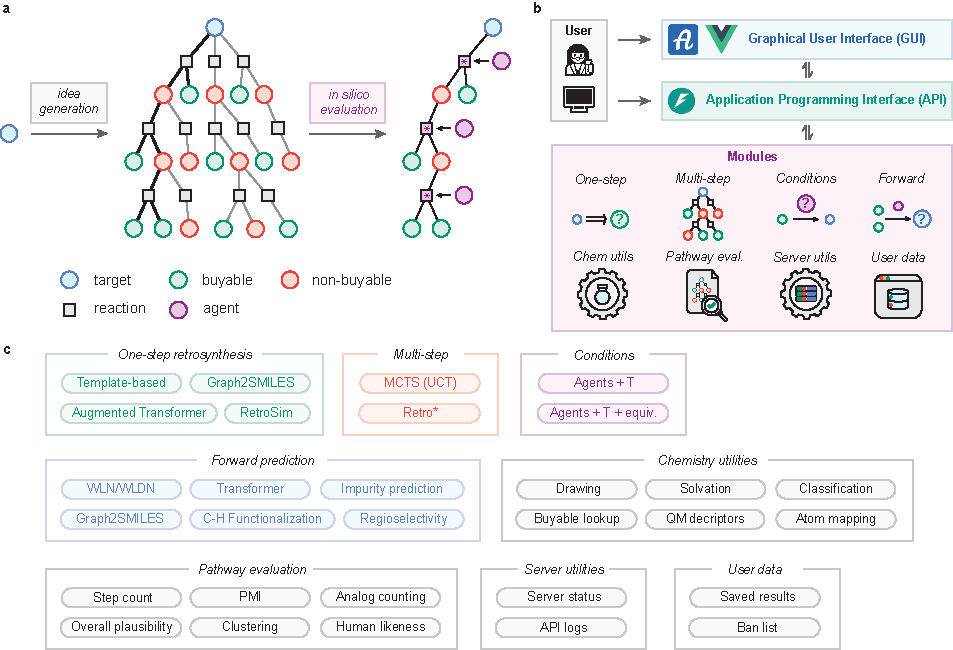
\includegraphics[width=1.0\textwidth]{media/0.Overviewfix.pdf}
\caption{ASKCOS overview. \textbf{a)} The typical target-oriented synthesis workflow for which ASKCOS is designed. A target molecule (blue circle) is recursively expanded retrosynthetically until buyable starting materials (green circles) are reached. Agents/conditions can be predicted for each proposed reaction, which can then undergo further evaluation, e.g., to anticipate reaction products. \textbf{b)} High-level flowchart for ASKCOS usage. A user can either interact via the graphical user interface or programmatic endpoints, which call various prediction modules. \textbf{c)} Summary of modules available in ASKCOS, which fall under themes including one-step retrosynthesis (green), multi-step search (red), condition recommendation (purple), reaction outcome prediction (blue), as well as utilities and supplementary capabilities (black). The modularity of the software design enables the straightforward extension of functionality (e.g., to new data-driven models) as they are developed in a research setting and made production-ready.}\label{fig_overview}
\end{figure}

\section{Results}\label{results}

\subsection{One-step retrosynthetic expansion}\label{results_one_step}

The one-step retrosynthetic expansion engine lies at the core of retrosynthetic analysis in ASKCOS. Given a target molecule, a list of candidate precursors is first predicted with user-specified one-step model(s). A fast plausibility filter based on the in-scope filter described by \citet{segler_planning_2018} removes unlikely precursors, and the remaining list is reranked based on buyability and complexity (e.g., by heavy atom count, ring count, or by SCScore~\citep{coley_scscore_2018}). Thereafter, the candidates undergo a series of optional post-processing steps. Because several predictions from the list of candidate precursors may correspond to highly similar strategies (e.g., differing only by leaving groups), precursors can be clustered based on their structures or reaction classes to return a diverse set of suggestions to the user; atom mapping and template extraction can be performed on reactions proposed by template-free model(s), which help check the chemical validity of the suggestions; precursors can be filtered or grouped based on which atoms are involved in the reaction centers; selectivity checks can automatically flag reactions with potential regioselectivity issues.

\begin{figure}[h!]
\centering
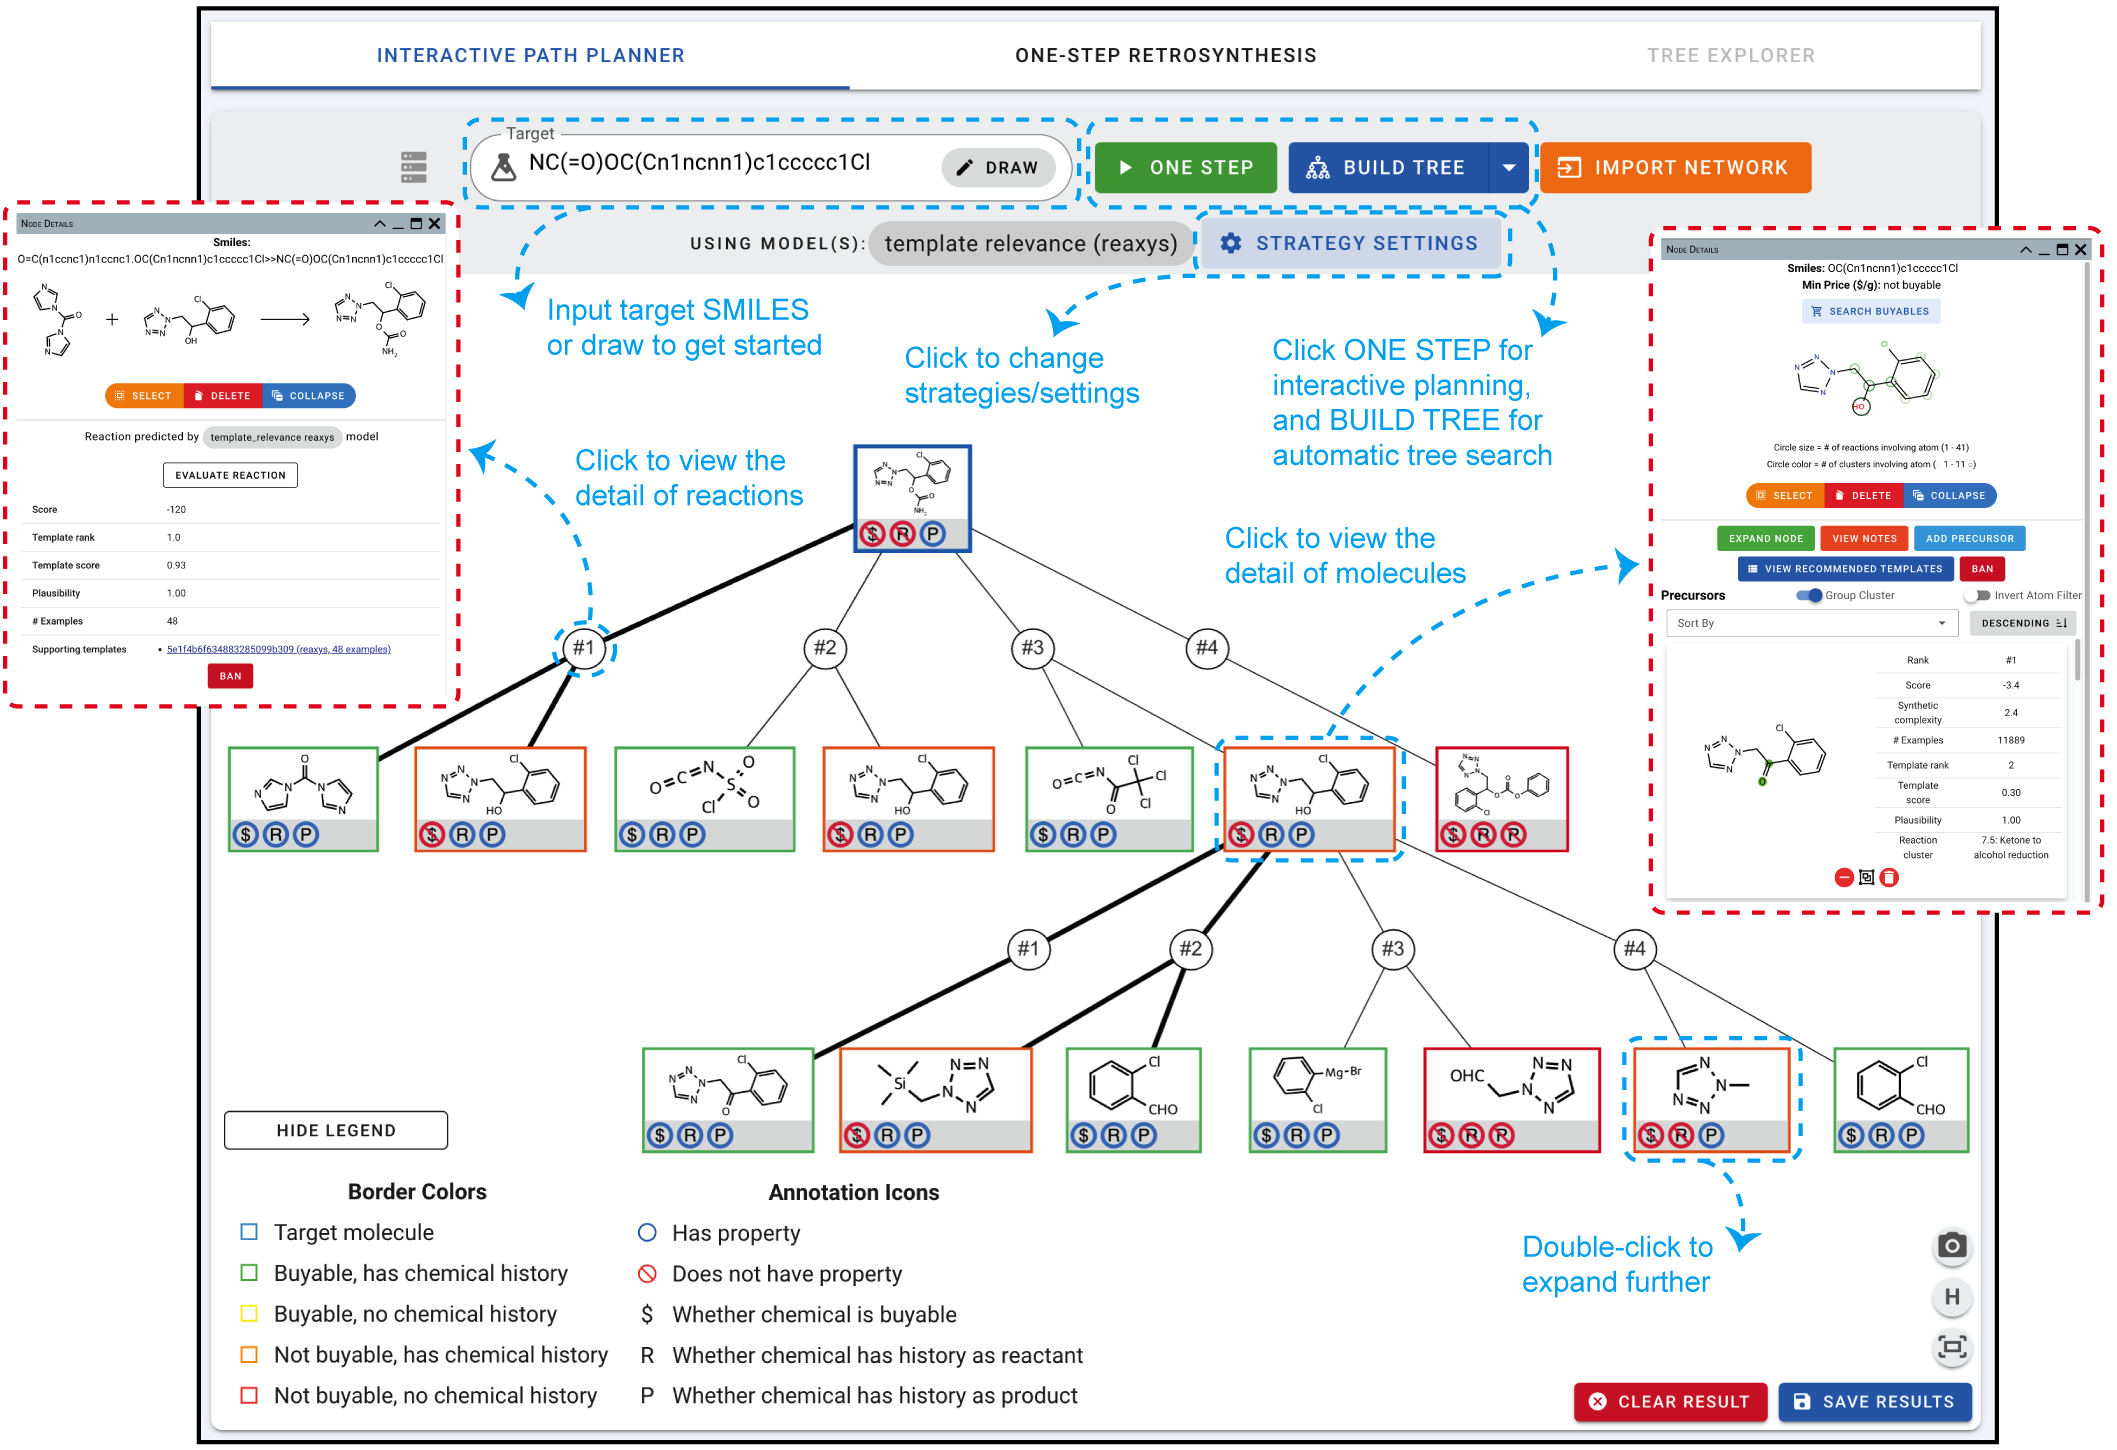
\includegraphics[width=1.0\textwidth]{media/1.IPP.png}
\caption{Annotated screenshot of the interactive planning canvas in ASKCOS. The input target molecule shown is cenobamate, a drug for partial-onset seizures, defined by entering the SMILES string \texttt{NC(=O)OC(Cn1ncnn1)c1ccccc1Cl} in the search bar or using an external name resolver if permitted by security policies. An interactive retrosynthetic search can be initiated with the \texttt{ONE STEP} button. An automated multi-step retrosynthetic search can be initiated with the \texttt{BUILD TREE} button. Search settings for both modes can be set with the \texttt{STRATEGY SETTINGS} button. Here, results are shown for an interactive search performed using the template-based single step model trained on the Reaxys dataset. The top 4 suggestions by the model are displayed on the canvas. A legend for the frame colors is displayed at the bottom left of the page. The displayed two-tier tree was generated by following the initial single step expansion of the target molecule with the expansion of one of the suggested precursors. Additional retrosynthetic expansions can be performed by double clicking on a chemical node. The chemical node info window provides users with additional information and actions (e.g., adding a comment for that chemical or banning it from future suggestions). If a one-step model has already been used to suggest precursors for that chemical, the node info window displays (right inset, red dashed frame) suggested precursors and allows users to sort or filter these suggestions using a variety of metrics (e.g., score, synthetic complexity, number of rings). A reaction node info window (left inset, red dashed frame)  provides users with information about the suggested reaction, including predicted scores and database precedents if they exist. The window also allows users to perform actions on the node such as removing or hiding it. Results can be saved, exported, or reorganized into different graphical views using additional tools in the bottom-right of the canvas.}\label{fig_ipp}
\end{figure}

\subsection{Interactive planning with the template relevance model}\label{results_ipp_template}

% CWC suggestion: paragraph on the scientific aspects of what ASKCOS includes

The use of reaction templates to suggest retrosynthetic disconnections has remained a popular choice since its origination in the early CASP tools of the 1960s~\citep{corey_computer-assisted_1969,wipke_simulation_1978,corey_computer-assisted_1972}. Template-based models within ASKCOS follow the neural-symbolic approach of \citet{segler_neural-symbolic_2017} wherein a policy network is trained to rank which templates appear most \emph{strategic} and \emph{chemically plausible} given the target. ASKCOS contains a variety of such models trained to use template sets derived from reactions in Pistachio~\citep{Pistachio}, CAS Content~\citep{CASContent}, USPTO~\citep{lowe_extraction_2012}, and Reaxys~\citep{Reaxys} using RDChiral~\citep{coley_rdchiral_2019} (see Section \nameref{methods}). Specialized models trained on enzymatic reaction data in BKMS~\citep{BKMS} and a specialized ``ring-breaker'' Pistachio model are also available and described in \citet{levin_merging_2022} and \citet{thakkar_ring_2020}, respectively. Because template-based models propose candidate precursors using templates extracted from published reactions, model suggestions can be traced back to reaction precedents and are therefore somewhat explainable.

% CWC suggestion: paragraph on how this is accessed/used from within ASKCOS as a software tool

Figure \ref{fig_ipp} shows a sample planning step with the original template-based model trained on Reaxys in 2016 in the \emph{Interactive Path Planner (IPP)}. The target is specified by a simplified molecular input line entry system (SMILES) string~\citep{weininger_smiles_1988} but can also be defined by drawing its structure with Ketcher or by common name using the PubChem API~\citep{PubChemAPI}. One-step expansion can then be triggered by pressing the green button. The top few (5 by default) suggestions will be added to the canvas as the child nodes of the target, with circles representing the reaction nodes and rectangles representing the molecule nodes. Clicking on the nodes display more context-specific details (shown as inset figures in red dotted lines in Figure \ref{fig_ipp}) and provide access to additional features, such as banning the reaction/molecule (thereby preventing them from appearing in future searches) or deleting/collapsing all child nodes of that node. Reaction nodes report the template scores (i.e., the template probabilities returned by the model), plausibility (evaluated by the fast binary filter as mentioned in Section \nameref{results_one_step}), and links to template details (which include links to the reaction precedents that the templates were extracted from). 

Each reaction can be analyzed further with the \texttt{EVALUATE REACTION} button, such as recommending conditions for the reaction or predicting reaction outcomes (see Sections \nameref{results_condition} and \nameref{results_forward} for details). Molecule nodes report their price and are additionally color-coded to reflect whether they are buyable or appear in known reactions stored in a reference database, as explained in the bottom-left IPP legend. Molecule node-specific features are also available, including expanding the nodes, adding and saving notes, and viewing recommended templates for the molecule. Once molecule nodes are expanded, their node details additionally list \emph{all} predicted precursors. These precursors can then be sorted according to different criteria (e.g., heuristic scores, synthetic complexity, number of precedents), grouped into clusters (if already clustered as mentioned in Section \nameref{results_one_step}), or filtered by reaction center by selecting the green-circled atom in the rendering of the molecule. Specific precursors can be added or removed from the canvas with the green \texttt{+} button or the red \texttt{-} button, respectively. 

After this first expansion of the target molecule, it is up to the user to decide which molecule node(s) to expand further, hence the \emph{interactive} nature of this view. For instance, users can choose a non-buyable molecule to expand next and continue this process until an appropriate pathway is identified. Precursors can be added to the molecule manually with the \texttt{ADD PRECURSOR} button if a user wishes to supplement model predictions with their own ideas. The explored network and notes can be saved to a user's profile for future access or exported as a JSON file for offline processing. 

\subsection{Interactive planning with multiple models, including template-free models}\label{results_ipp_multiple}

% CWC suggestion: paragraph on the scientific aspects of what ASKCOS includes

There is an abundance of one-step retrosynthetic models reported in the past several years that forgo the use of templates and instead learn to predict reactant structures from product structures in a more flexible end-to-end manner. ASKCOS currently contains four categories of one-step strategies, including Transformer~\citep{lin_automatic_2020,tetko_state---art_2020,schwaller_molecular_2019}, Graph2SMILES~\citep{tu_permutation_2022}, Retrosim~\citep{coley_computer-assisted_2017}, and the aforementioned template relevance strategy~\citep{segler_neural-symbolic_2017}. Transformer and Graph2SMILES use template-free approaches and model retrosynthesis as SMILES-to-SMILES and graph-to-SMILES translation tasks, respectively. Retrosim offers a retrieval-based, learning-free approach in which reactions are suggested based on analogy to most-similar precedents. Each model may exhibit distinct strengths and failure modes not reflected in their quantitative performance on standard benchmark tasks (Table~\ref{tab1_one_step}). For this reason, ASKCOS supports the consolidation of recommendations from multiple strategies; when multiple models recommend the same precursors, this can be interpreted as a sign of confidence in that recommendation.

% CWC suggestion: paragraph on how this is accessed/used from within ASKCOS as a software tool

Mixing and matching different one-step strategies is performed within the \texttt{STRATEGY SETTINGS} menu (Figure \ref{fig_ipp}). Different strategies are queried in sequence and combined results are de-duplicated before appearing on the page. Each strategy has its own settings, such as the maximum number of templates to be applied for the template relevance model and the training set to use. When viewing node details, suggested reactions from template-free and Retrosim models contain different metadata (e.g., Retrosim results display the reaction precedents if that information is included on deployment). When multiple models predict the same precursor, the metadata from all models are merged to show all template and/or reaction precedent information where applicable. Most of these strategies can be retrained using new reaction databases, e.g., proprietary collections from an internal electronic lab notebook system, which may provide better coverage of different reaction and substrate types.

\begin{table}[h!]
\caption{Previously reported top-k accuracies (\%) of one-step models on two commonly-used benchmark datasets: USPTO-50k~\citep{schneider_whats_2016} and USPTO-full~\citep{dai_retrosynthesis_2019}.}\label{tab1_one_step}
\begin{tabular*}{\textwidth}{@{\extracolsep\fill}llcccccc}
\toprule
& & \multicolumn{3}{@{}c@{}}{USPTO-50k} & \multicolumn{3}{@{}c@{}}{USPTO-full} \\
\cmidrule{3-5}\cmidrule{6-8}
Model name & Type & Top 1 & Top 10 & Ref. 
& Top 1 & Top 10 & Ref. \\
\midrule
Template relevance
& Template-based    
& 45.2 
& 83.5 &~\citep{seidl_improving_2022} 
& 35.8 
& 60.8 &~\citep{dai_retrosynthesis_2019} \\
Retrosim
& Template-based    
& 37.3 
& 74.1 &~\citep{coley_computer-assisted_2017}
& 32.8
& 56.1 &~\citep{dai_retrosynthesis_2019} \\
Transformer w/o aug. 
& Template-free     
& 43.1 
& 78.7 &~\citep{lin_automatic_2020}
& 42.9 
& 66.8 &~\citep{zhu_dual-view_2023} \\
Transformer w/ aug. 
& Template-free     
& 53.2 
& 85.2 &~\citep{tetko_state---art_2020}
& 44.4 
& 73.3 &~\citep{tetko_state---art_2020} \\
Graph2SMILES 
& Template-free     
& 52.9 
& 79.5 &~\citep{tu_permutation_2022}
& 45.7 
& 63.4 &~\citep{tu_permutation_2022} \\
\botrule
\end{tabular*}
\footnotetext{Note: for the template relevance model, accuracies on the original NeuralSym model are reported. Best values from multiple references are recorded. Transformer w/ aug. refers to the variant where equivalent reaction SMILES are used to \emph{augment} the training set, which is a known empirical technique for boosting accuracy~\citep{bjerrum_smiles_2017}. Due to the vast amount of literature related to Transformer and SMILES augmentation, we did not attempt to do an exhaustive literature survey for Transformer-based models.}
\end{table}

\subsection{Automatic multi-step planning with the Tree Builder}\label{results_tree_builder}

\begin{figure}[h!]
\centering
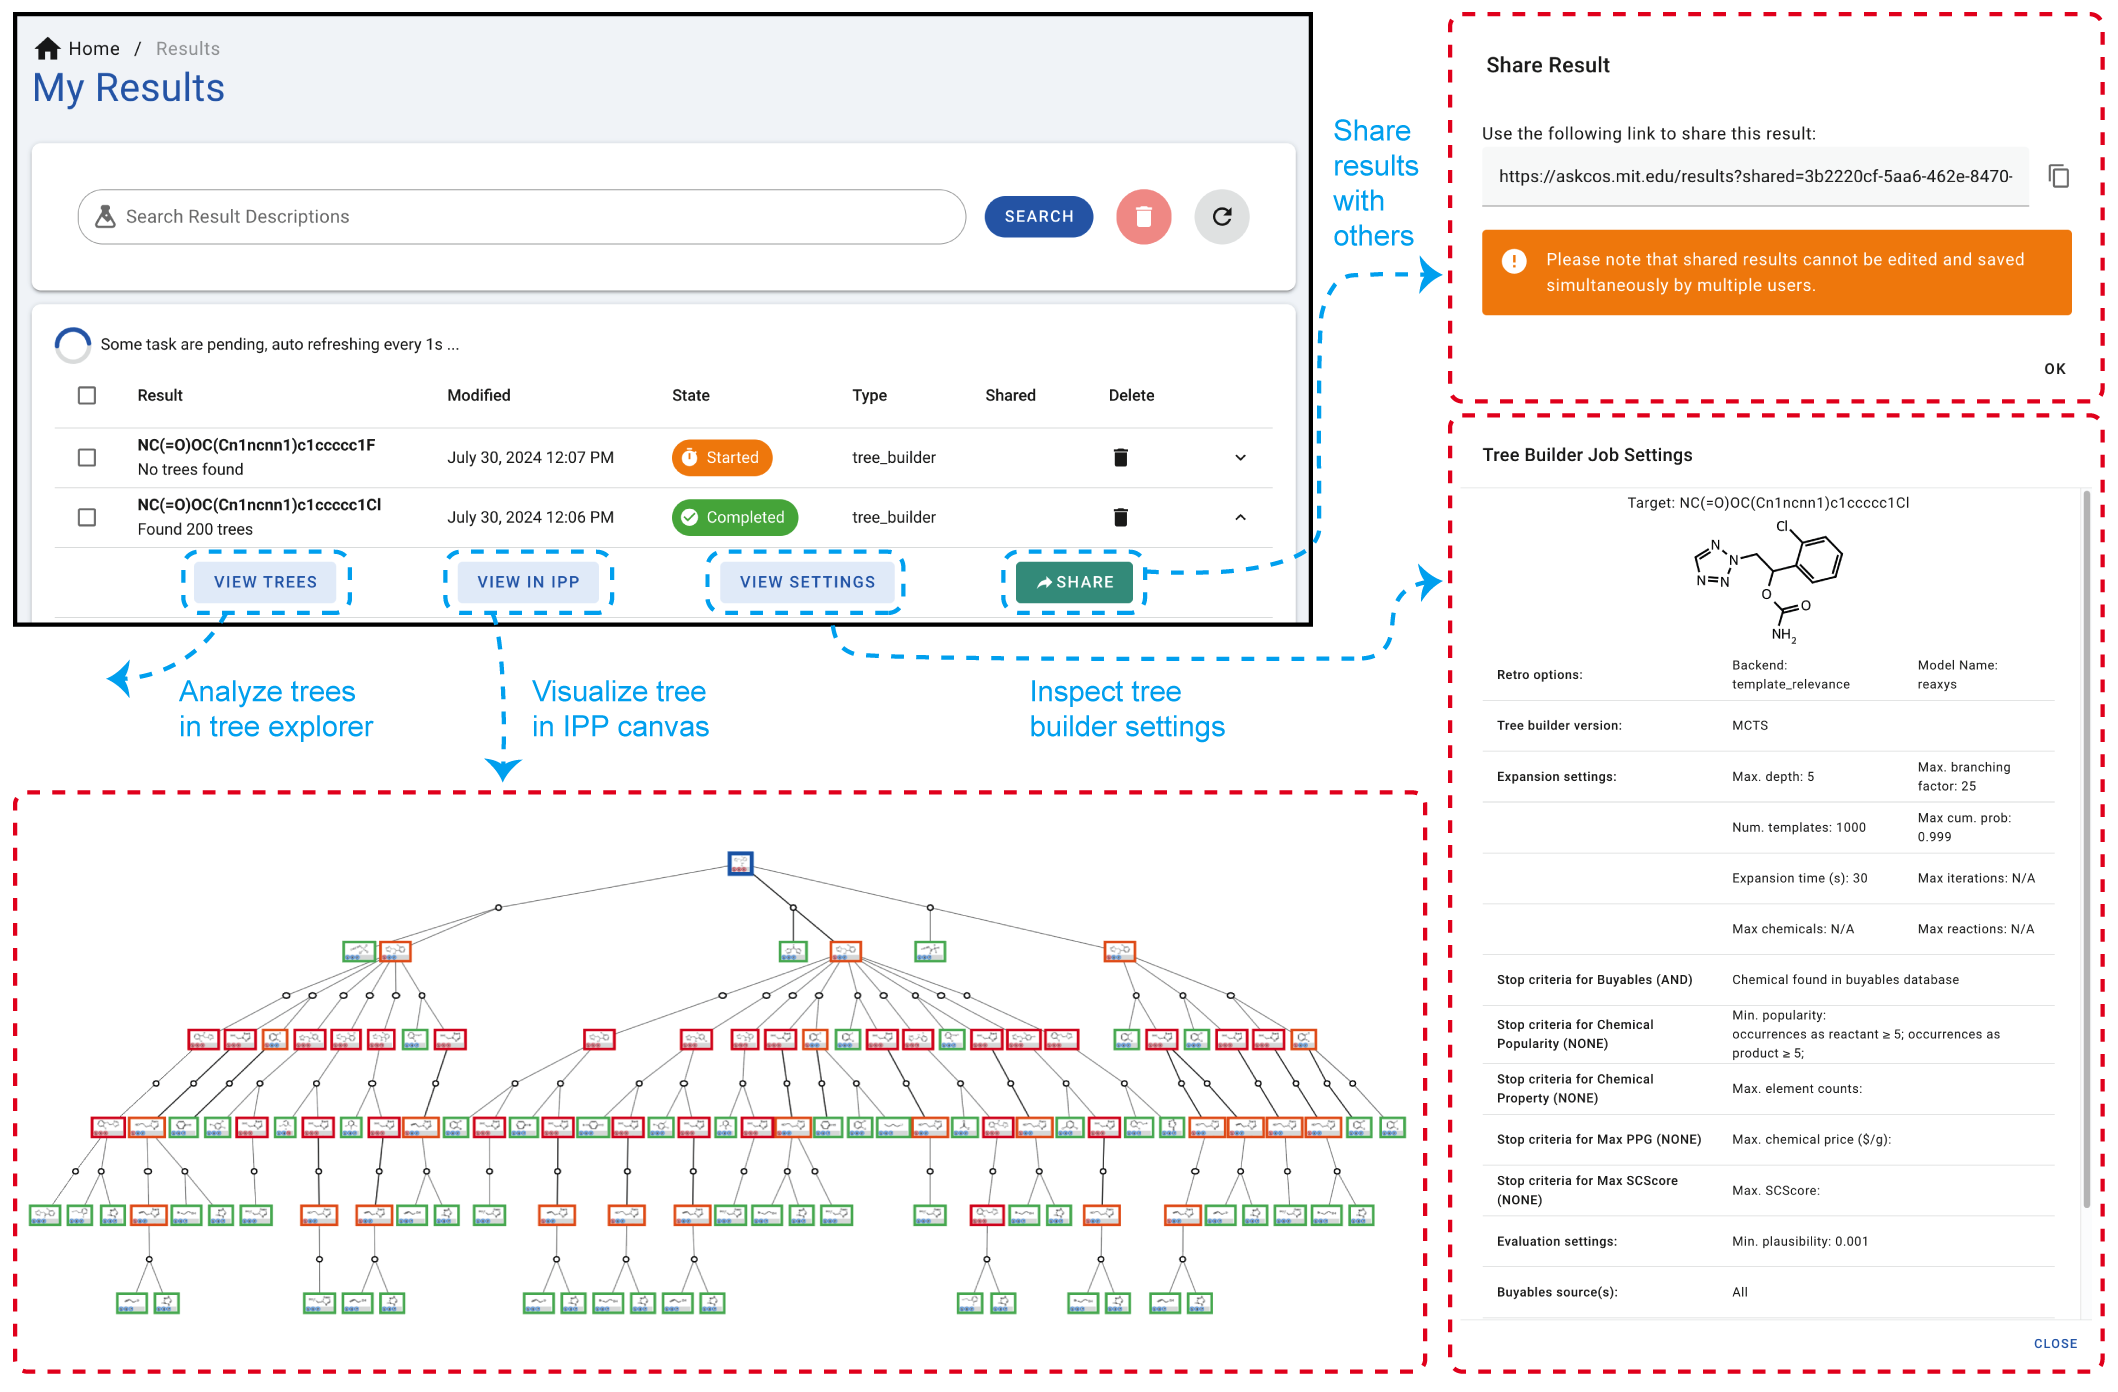
\includegraphics[width=1.0\textwidth]{media/2.TreeResult.png}
\caption{Annotated screenshot of tree search results in ASKCOS. The Tree Builder job can be initiated with the \texttt{BUILD TREE} button on the interactive path planning page. In \texttt{My Results} page, the status for the Tree Builder job is shown as \texttt{Started}. Once the job is complete, the status changes to \texttt{Completed}, and the trees found can be visualized/analyzed in the Tree Explorer (\texttt{VIEW TREES}) or the IPP canvas (\texttt{VIEW IN IPP}). The settings used for the Tree Builder job can be viewed with the \texttt{VIEW SETTINGS} button, and the results can be shared with others with the \texttt{SHARE} button. Here, the Tree Builder job for the target molecule \texttt{NC(=O)OC(Cn1ncnn1)c1ccccc1Cl} is performed using the MCTS algorithm with the template-based single step model trained on the Reaxys dataset, using a maximum depth of 5, a maximum branching factor of 25, and an expansion time of 30s (right bottom inset, red dashed frame). The results can be visualized in the IPP canvas {(left bottom inset, red dashed frame)}.}\label{fig_tree_results}
\end{figure}

% CWC suggestion of same format: one paragraph on general sciency part, then one paragraph on the software part

In addition to interactive planning where users guide the selection of which molecule nodes to expand, \emph{automatic} planning can be more convenient, particularly when there are many target molecules of interest. Retrosynthetic searches can be run for thousands of targets through asynchronous requests, albeit at the expense of losing explicit control on the direction of expansion. Formally, automatic multi-step planning has been formulated as tree search or graph search problems. In each iteration of the search, a molecule is selected for one-step retrosynthetic expansion. New hypothetical reactions and their corresponding reactants are added to the search tree. This process is repeated until some termination criterion is reached, for example, until a synthetic pathway is found in which all starting materials are buyable. The well-known baseline algorithms include Monte Carlo tree search (MCTS)~\citep{segler_planning_2018,lin_automatic_2020}, Proof Number Search (PNS)~\citep{heifets_construction_2012,kishimoto_depth-first_2019} and A* Search~\citep{chen_retro_2020} which tend to be inspired by other artificial intelligence applications such as AlphaGo~\citep{silver_mastering_2016}. More recent work in the field on such search algorithms has mainly focused on improvement of selection policies, for example, with reinforcement learning~\citep{liu_retrosynthetic_2023, yu_grasp_2022,schreck_learning_2019, wang_towards_2020}, supervised learning~\citep{xie_retrograph_2022,zhao_efficient_2024, hong_retrosynthetic_2023}, or chemical heuristics~\citep{schwaller_predicting_2020, kreutter_multistep_2023}. A number of studies have also sought to improve the expansion policy by focusing on the one-step model in the context of multi-step planning~\citep{liu_fusionretro_2023,kim_self-improved_2021}. Others have approached synthesis planning outside of the typical tree search formulation, such as through sequence generation~\citep{shee_directmultistep_2024} or as a bidirectional search~\citep{yu_double-ended_2024}.

ASKCOS supports automatic planning through the \emph{Tree Builder} module which currently provides two search algorithms, MCTS~\citep{segler_planning_2018} and Retro*~\citep{chen_retro_2020}. Either can be selected from \texttt{STRATEGY SETTINGS}. After specifying the target in the IPP canvas, the user can click the \texttt{BUILD TREE} button in Figure \ref{fig_ipp} to initiate a Tree Builder job, which will run asynchronously in the background. A pop-up window will inform the user when the results are ready and available for viewing. All tree results can be found under the \texttt{My Results} page as shown on the top left corner of Figure \ref{fig_tree_results}, where the status of any result entry will change from \texttt{started} to \texttt{completed} once the Tree Builder job is finished. From here, the user can visualize the result either as a full retrosynthesis tree in the IPP canvas, or as individual routes in the Tree Explorer (see Section \nameref{results_pathway_analysis} for further analysis). The settings used for the job can be inspected, and the result can be shared via the green sharing button in Figure \ref{fig_tree_results}.

\subsection{Reaction condition recommendation}\label{results_condition}

\begin{figure}[h!]
\centering
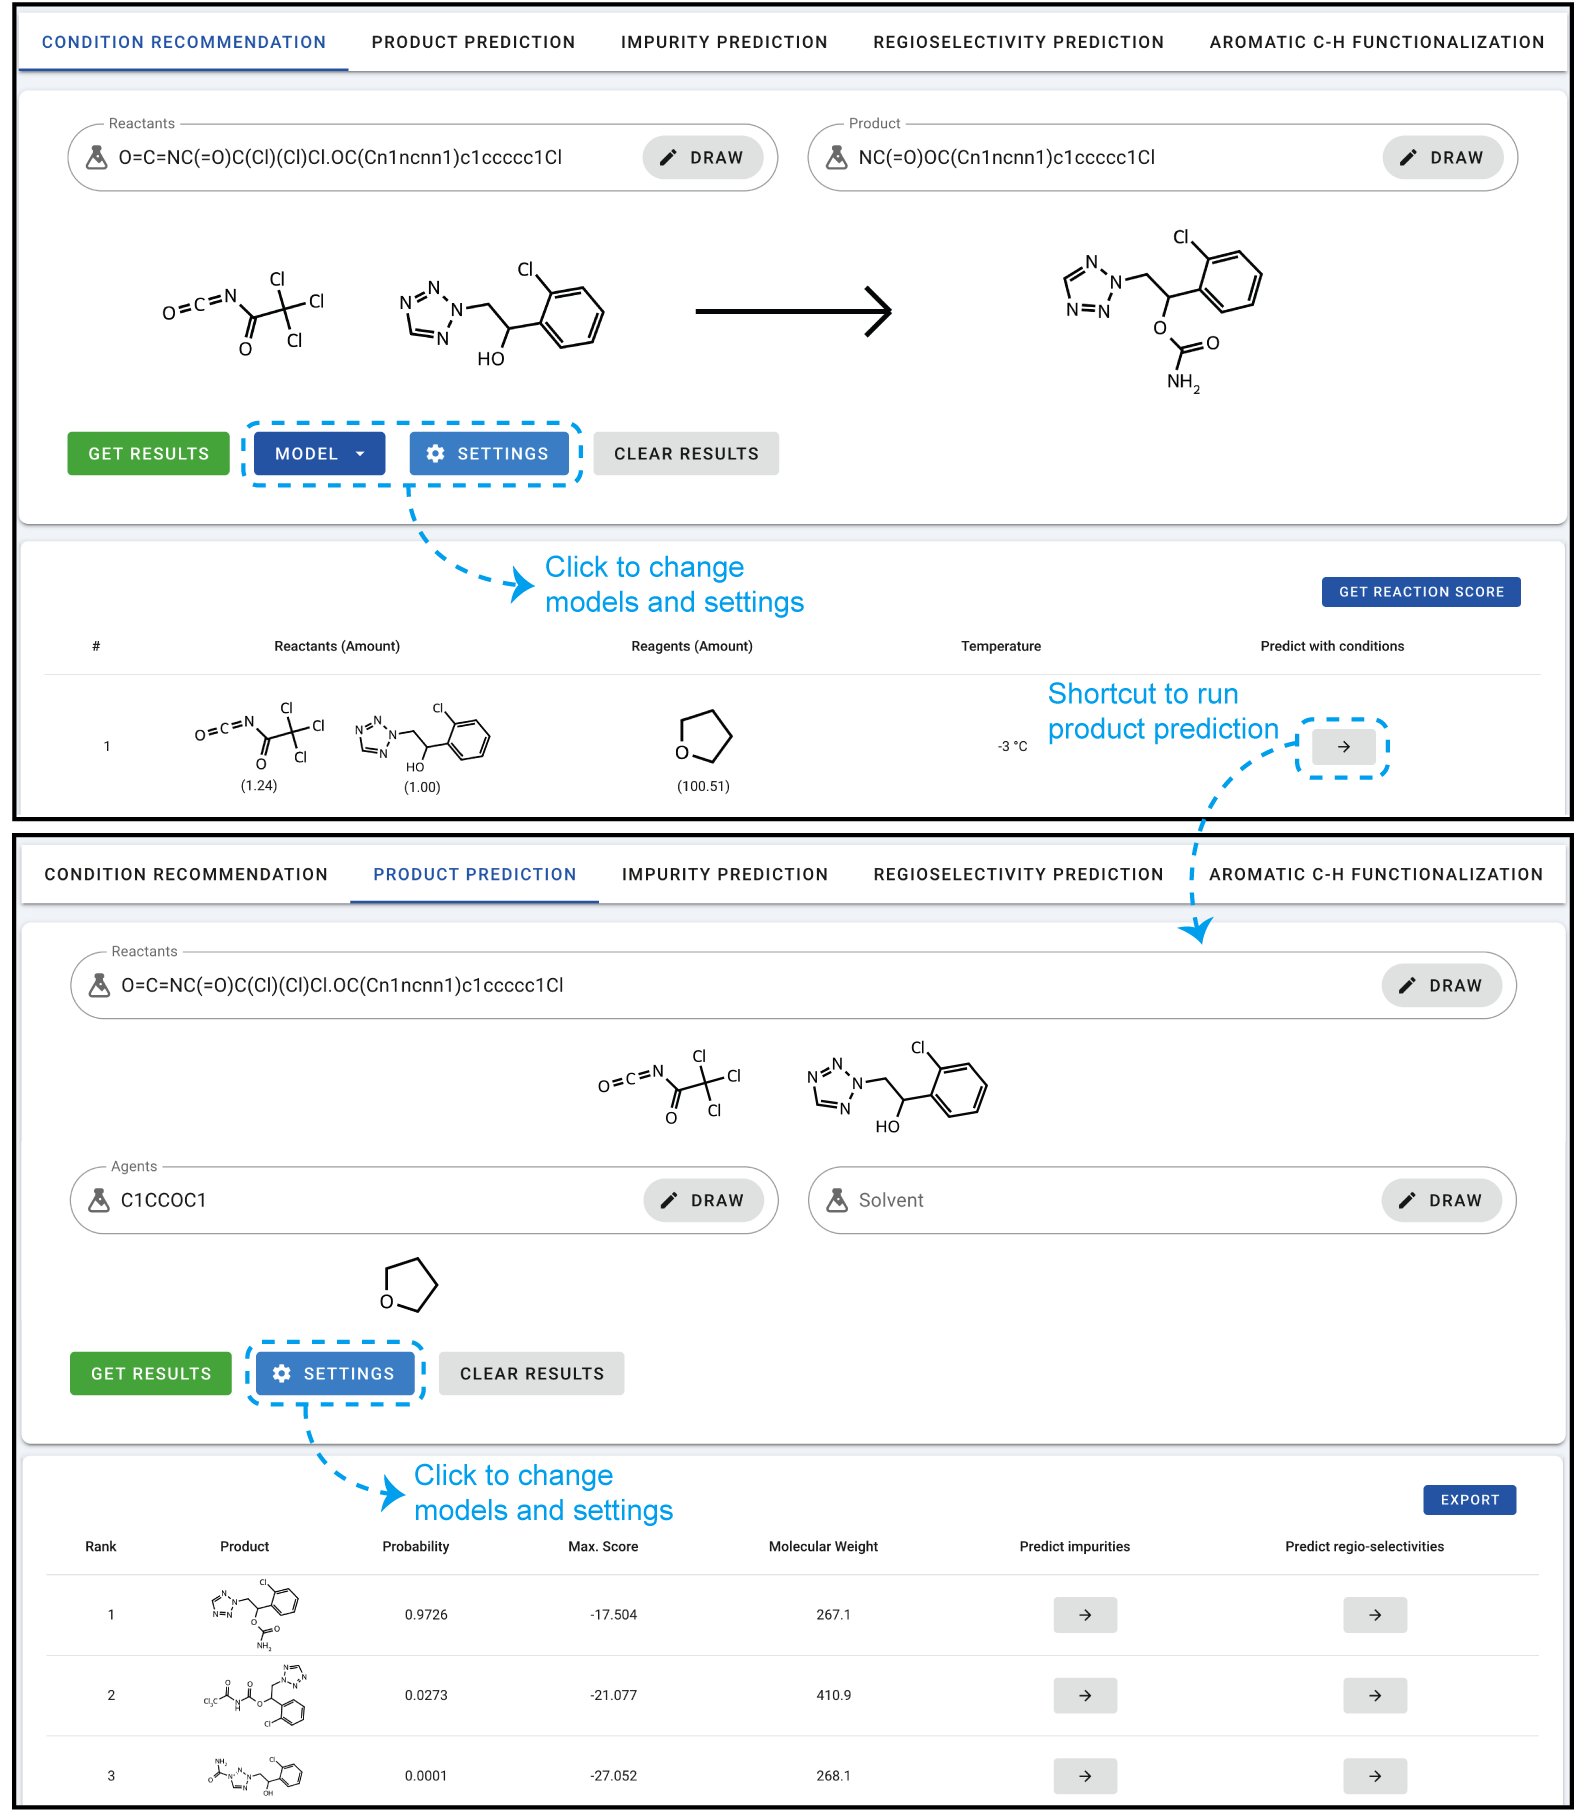
\includegraphics[width=1.0\textwidth]{media/3.Forward.png}
\caption{Annotated screenshot of the condition recommender (top) and the forward predictor (bottom) in ASKCOS. In the condition recommender, the SMILES strings of reactants and products are input in the \texttt{Reactants} and \texttt{Products} panels. Condition recommendation can be initiated with the \texttt{GET RESULTS} button. Prediction models and their training set can be set with the \texttt{MODEL} and \texttt{SETTINGS} buttons, respectively. Each proposed condition has shortcuts to run product prediction. In the forward predictor, the SMILES strings of reactants and agents are pre-populated using the shortcut from the condition recommendation page. Product prediction can be initiated with the \texttt{GET RESULTS} button. Prediction models and their training sets are chosen via \texttt{SETTINGS} button. Here, the results are shown for three predicted products with their probabilities, which should be interpreted only qualitatively. Each prediction has shortcuts to run impurity and regioselectivity prediction as additional evaluations.}\label{fig_forward}
\end{figure}

% The science (the task and the formulation)

The prediction of reaction conditions, including the identity of agents (catalysts, reagents, solvents) and operating conditions such as temperature and equivalence ratios, is an often overlooked aspect of synthesis planning. Condition recommendation is essential for any suggested reactions to be experimentally validated, and reaction outcomes are strongly influenced by reaction conditions. Reaction type specific data-driven models have been built, for example, to predict classes of solvent and catalyst for Michael additions~\citep{marcou_expert_2015}, ligands for Pd-catalyzed C-N coupling~\citep{li_making_2019}, and reaction contexts including temperature and pressure for four families of substrate-specific cross-coupling reactions~\citep{maser_multilabel_2021,kwon_generative_2022}. \emph{Global} models which are not specific to reaction families have also been developed using a variety of approaches, including multi-class classifier chains~\citep{gao_using_2018} and its variant using a Transformer encoder with SMILES inputs~\citep{wang_generic_2023},  retrieval-augmented prediction using text descriptions of similar reactions~\citep{qian_predictive_2023}, and a two-stage model with candidate generation and ranking as distinct steps~\citep{chen_enhancing_2024}. 

% The usage in ASKCOS

ASKCOS includes a data-driven condition recommendation model based on \citet{gao_using_2018} as well as a second version being developed in ongoing work which additionally predicts equivalence ratios. This model formulates condition recommendation in terms of four sub-problems (1) predicting agent identities as multi-label classification; (2) predicting temperature as binned classification; (3) predicting reactant equivalence ratios as multi-target regression; and (4) predicting agent equivalence ratios as multi-target regression. A screenshot of the condition recommendation page in ASKCOS is shown at the top of Figure \ref{fig_forward}. As with other pages, the reactants and product can be specified either by SMILES strings or by drawing. After generating model predictions by clicking on \texttt{GET RESULTS}, several different condition settings are displayed in a tabular format. The general layout of the reaction condition recommendation page is used across several other modules for consistency: the top panel is for the inputs and the bottom panel is for the prediction results; the model and settings can be modified by clicking on the blue buttons for \texttt{MODEL} and \texttt{SETTINGS}.

\subsection{Reaction outcome prediction}\label{results_forward}

% The science (the task and the formulation)

Another component of synthesis planning beyond retrosynthesis is the prediction of reaction outcome(s). In our workflows, these predictions mostly serve to identify chemically infeasible or unfavorable reactions, which the user can choose to prune from the synthesis tree in an interactive setting. Many data-driven approaches simplify this task as predicting the identity of the major product, making it equivalent to a molecule-to-molecule transformation. Similar to one-step retrosynthesis, some studies have formulated it as forward template prediction~\citep{coley_prediction_2017,chen_generalized-template-based_2022}, whereas later developments have been dominated by graph-edit based~\citep{coley_graph-convolutional_2019,sacha_molecule_2021}, electron-flow based~\citep{bradshaw_generative_2019,bi_non-autoregressive_2021}, and translation-based~\citep{schwaller_molecular_2019,tetko_state---art_2020,tu_permutation_2022,zhong_root-aligned_2022} template-free methods. Outcome prediction can answer more fine-grained questions about reaction outcomes, such as the site selectivity of aromatic C-H functionalization reactions~\citep{struble_multitask_2020} or other situations where multiple regioisomers appear possible based on reaction templates~\citep{guan_regio-selectivity_2021}. Another application of outcome prediction is the analysis of potential impurities. When impurities are defined as the minor products of the main reactions or the products of side reactions, they can be predicted by considering several predicted reaction outcomes with lower probabilities or by predicting the outcomes of new reactant sets containing a product of the original reactions (i.e., anticipating potential over-reaction).

% The usage in ASKCOS

The major product prediction page in ASKCOS is shown in the bottom of Figure \ref{fig_forward}. In this specific example, the top outcome is carbamate formation arising from nucleophilic attack of the alcohol into the isocyanate (followed by hydrolysis~\citep{hirama_carbamate_1982}) with a probability of 0.9726. Non-hydrolyzed product and nucleophilic attack by a tetrazole nitrogen are predicted to be the second and third most likely products, but with lower probabilities of 0.0273 and 0.0001, respectively. Past studies have shown these probabilities to correlate with accuracy \emph{on average} but may not be a robust measure of confidence for a particular result~\citep{coley_graph-convolutional_2019,schwaller_molecular_2019,neves_global_2023}. Modules for impurity prediction, regioselectivity, and C-H site-selectivity are accessible via other tabs on the same page. The impurity prediction module relies on the major product predictor and considers minor products, over-reaction, dimerization, solvent adducts, and subsets of reactants; the details of regio- and site-selectivity predictions are reported in \citet{guan_regio-selectivity_2021} and \citet{struble_multitask_2020}, respectively.

\subsection{Pathway scoring and ranking}\label{results_pathway_analysis}

\begin{figure}[h!]
\centering
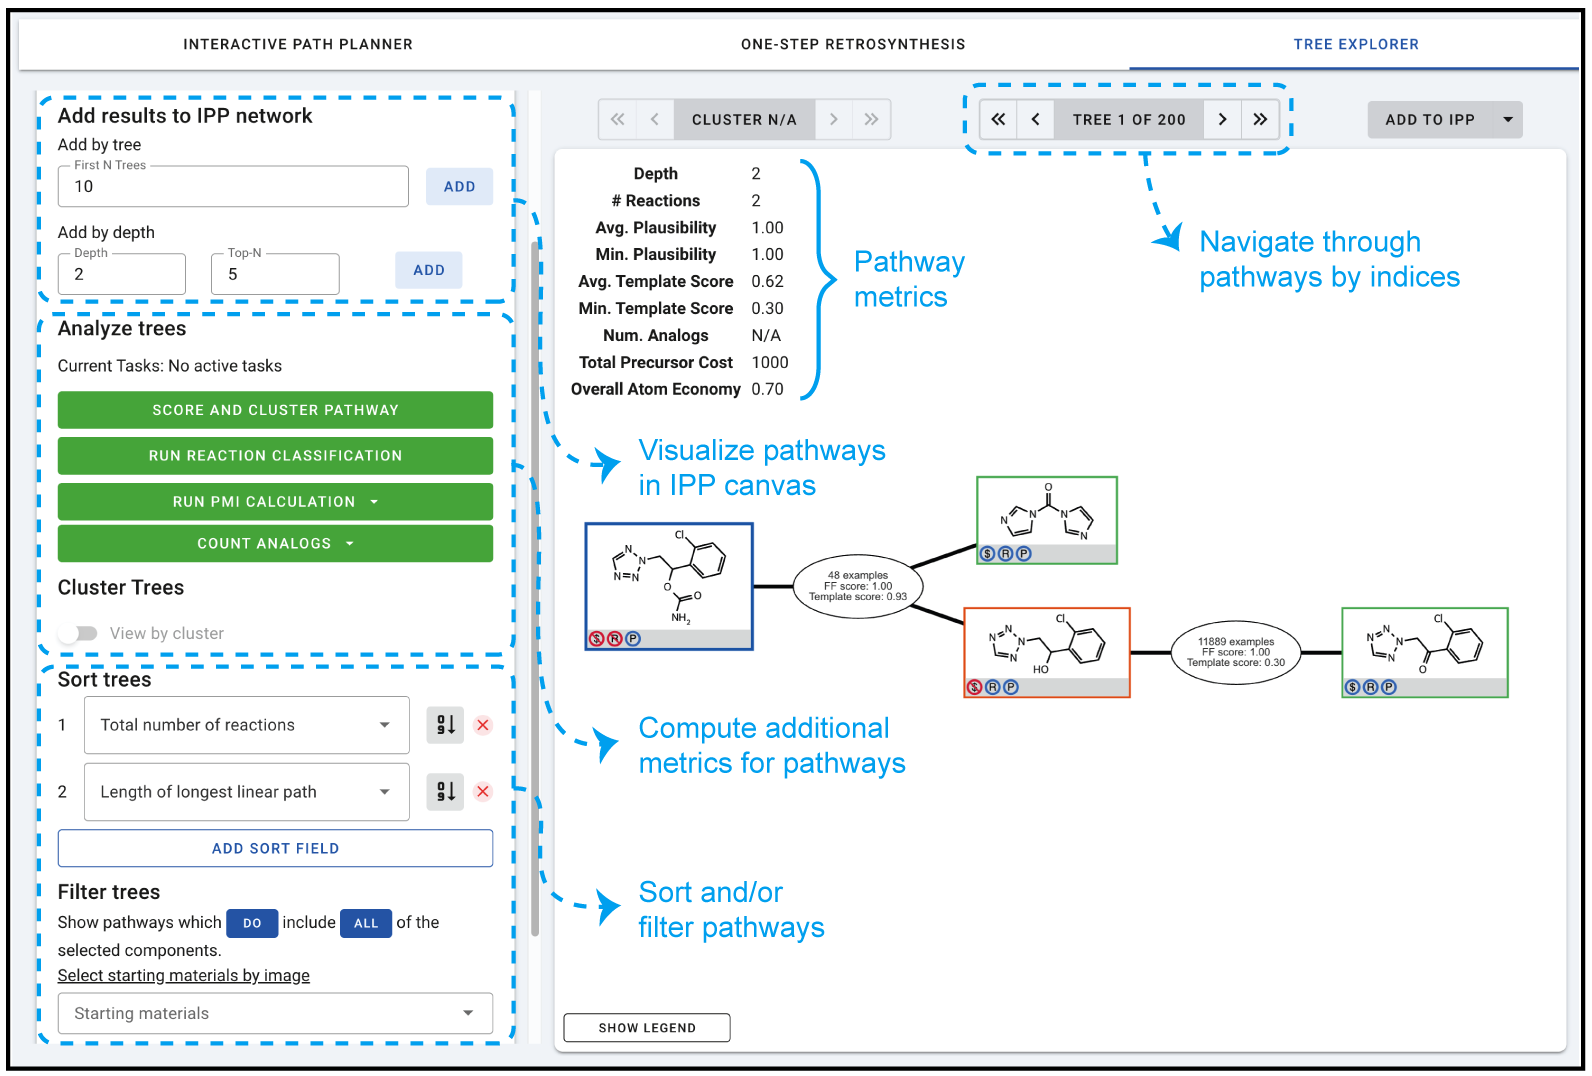
\includegraphics[width=1.0\textwidth]{media/4.TreeExplorer.png}
\caption{Annotated screenshot of the Tree Explorer in ASKCOS. One of 200 routes returned for the target molecule cenobamate is displayed in the main panel (right) of the window. Pathway metrics for the route are shown in the top left corner of the main panel. The left panel provides users with additional actions to perform on the returned synthetic routes. Users can transfer information from the Tree Builder to the Interactive Path Planner to continue exploring retrosynthetic suggestions beyond what was returned (top); users can initiate longer-running pathway-level scoring calculations (middle); finally, users can sort or filter the discovered routes based on various calculated metrics or the presence or absence of specific starting materials and intermediates (bottom). }\label{fig_tree_explorer}
\end{figure}

When many putative synthetic pathways are found for a target molecule, a new challenge arises: to identify the routes that best satisfy a \emph{chemist's }goals, not merely to identify \emph{any} route. It is impractical to triage routes manually when the number of suggestions becomes too large. Strategically similar pathways can first be clustered or grouped based on trained pathway embeddings~\citep{mo_evaluating_2021} or the reactions types they involve (e.g., using NameRxn~\citep{NameRXN} categories or approximations thereof). Pathway-level evaluations then help prioritize promising synthetic routes, though there are many criteria by which a synthetic pathway could be judged~\citep{hoffmann_ranking_2009}. Simple, readily-calculable metrics include step count, longest linear sequence, atom economy, cost of starting materials, or diversifiability based on an estimate of the size of an analog space achieved through building block enumeration~\citep{levin_computer-aided_2023}. More complex metrics that may be derived from other predictive models include estimates of human likeness~\citep{mo_evaluating_2021}, overall perceived likelihood of feasibility, pathway greenness based on solvent usage~\citep{wang_towards_2020}, and process mass intensity (PMI). Assessing purification/isolation requirements in a robust manner remains elusive~\citep{kuznetsov_extractionscore_2021}.

Pathway evaluation in ASKCOS is intended to be performed on pathways returned by the Tree Builder and is accessible from the results page by clicking \texttt{VIEW TREES} as shown in Figure \ref{fig_tree_results}. Since none of the aforementioned evaluation criteria is perfect or sufficient on its own, ASKCOS makes all of them available as part of the \emph{Tree Explorer} (Figure \ref{fig_tree_explorer}), with operations and options on the left panel and the canvas on the right for displaying the pathway with its metrics. In this specific example, 200 pathways have been returned (the default maximum); the first pathway is shown along with automatically-calculated metrics such as the depth, the average plausibility, and the analog count of the pathway. The left panel is organized into three sections that allow the user to visualize multiple best-ranked pathways in the IPP canvas; calculate additional evaluation metrics on-request (rather than automatically due to their computational cost); and sort or filter pathways, e.g., based on certain starting materials of interest.

\subsection{Utilities and supplementary predictive models}\label{results_utilities}

% The "science" and then the "usage". This section is somewhat miscellaneous so we can be a bit more flexible about the organization.

Beyond these ``core'' synthesis planning capabilities, ASKCOS contains additional complementary tools. These include basic drawing functionality (\texttt{Drawing}) and buyable building block search by SMILES or SMARTS (\texttt{Buyable Look-up}). The latter makes use of a predefined commercial catalog that is easily customizable when ASKCOS is deployed. The utilities page also offers two additional machine learning models for solvation prediction (\texttt{Solubility Prediction} and \texttt{Solvent Screening})~\citep{vermeire_predicting_2022} and the prediction of atom- and bond-level descriptors calculated by DFT (\texttt{QM Descriptor})~\citep{guan_regio-selectivity_2021,li_when_2024}. Solubility prediction is part of a long-term goal of improving the relevance of CASP for process chemistry~\citep{griffin_opportunities_2023} as it helps guide the selection of solvents for reactions, liquid-liquid extractions, or crystallizations. ML-estimated QM descriptors can be used as features by other predictive models~\citep{stuyver2022quantum} or standalone, e.g., for human assessment of selectivity. 

The pages for solubility prediction, solvent screening, and QM feature prediction are organized under the \texttt{Utilities} tab, each with a standard layout as in Figure \ref{fig_forward}. Solubility prediction requires a solute,  solvent, and temperature as inputs; solvent screening expects a single solute, a list of solvents, and a list of temperatures; QM prediction needs the SMILES of the target molecule. The screenshots of these pages are shown in Supplementary Figure \ref{fig_solubility_prediction}, \ref{fig_solvent_screening} and \ref{fig_qm_descriptors}, with more detailed explanation on the theoretical aspect and usage in Supplementary Sections \nameref{results_solubility} and \nameref{results_qm}.

\section{Discussion}\label{discussion}

% from submission guideline of Nature Synthesis: The Results section may be divided by topical subheadings, but the Discussion section should be succinct and **may not contain subheadings**

% \subsection{Adoption and use}

As a broad, extensible software suite for synthesis planning, ASKCOS has been adopted by various organizations within and beyond the context of the MLPDS consortium. While not all usage of ASKCOS is publicly described, several use cases where ASKCOS has aided chemists' workflows have been discussed in the 2020 review by \citet{struble_current_2020}. Particularly well-received features include the interactive planning mode when automatic tree search fails, as well as the possibility for retrosynthetic suggestions to be linked back to literature precedents. ASKCOS has helped serve as a foundation for components of AiZynthFinder~\citep{genheden_aizynthfinder_2020,shields_aizynth_2024} (e.g., in its template extraction strategy). Discovery chemists from Janssen have made use of various modules in ASKCOS at the lead optimization stage. In particular, the one-step retrosynthesis API helped narrow a library of 222k alcohols to 15.7k on the basis of synthesizability~\citep{seierstad_novel_2021}. Pfizer has reported the use of ASKCOS to augment human ideas in their internal graph databases~\citep{avila_chemistry_2024}, and Syngenta has incorporated ASKCOS as one of several idea generation tools when comparing synthetic routes \cite{pasquini2023linchemin}. Beyond the industrial setting, various researchers have used ASKCOS to propose synthetic routes for candidate protease inhibitors~\citep{soukaina_design_2024} and other potential anti-COVID-19 drugs~\citep{qi_optimized_2023}.

% \subsection{Managing expectations of CASP tools}

As is true of other computational tools, most if not all of the functionalities in ASKCOS aim to \emph{assist} and not replace expert chemists. Ultimately, these models are influenced by the data on which they are trained and may recapitulate popular patterns and trends in data (albeit in useful ways) without understanding the underlying physical sciences. The interpretability of our models fall on a wide spectrum. For the one-step retrosynthesis models, for example, template-based approaches ensure traceability to literature precedents. In contrast, translation-based approaches make predictions in a more black-box manner, which can be creative but to the extent of being alchemical, e.g., by inappropriately adding atoms in the generated SMILES. We refer the reader to individual manuscripts for each prediction module for more in-depth discussions on their strengths and limitations. 

% CWC note: I think we need more specific cross-referencing of figures in the SI to make this paragraph feel stronger. I've put placeholder "\#" in places where I think this would help. This also makes it sound more like we ran an EXPERIMENT and are reporting RESULTS in the SI, even if it's subject to only qualitative interpretation. 
As an illustration of how ASKCOS can be used as an assistive tool, we conduct a synthesis planning exercise, which is described further in Supplementary Section \nameref{results_fda}. We start with automatic retrosynthetic planning using the Tree Builder for all targets. Using typical search settings with template relevance models trained on Reaxys and Pistachio, the default buyable database (consisting of a few hundred thousand molecules from eMolecules~\citep{EMolecules}, Sigma Aldrich~\citep{SigmaAldrich}, LabNetwork~\citep{LabNetwork}, Mcule~\citep{Mcule}, and ChemBridge~\citep{ChemBridge}), and a limit on the number of chemical nodes in the search tree of 5000, hypothetical retrosynthetic pathways are found for many of the targets. Sample shortest routes are presented in Supplementary Figures \ref{fig:fda_study_1}, \ref{fig:fda_study_2}, \ref{fig:fda_study_3}, and \ref{fig:fda_study_4} \emph{exactly as returned} along with the top-1 proposed conditions from the V1 condition recommender. We then demonstrate the use of additional modules in ASKCOS for further analysis when proposed steps are counter-intuitive or appear implausible, e.g., by cross-referencing literature precedents or examining lower-ranked suggested conditions. Thereafter, we show how the flexibility of ASKCOS helps us handle the cases where automatic planning with typical settings fails, by providing a variety of tree search options, and more importantly, a user-friendly interface to directly modify proposed routes. Additional example pathways proposed by ASKCOS from three re-runs with manual edits where appropriate are shown in Supplementary Figures \ref{fig:fda_study_interesting_1}, \ref{fig:fda_study_interesting_2}, and \ref{fig:fda_study_interesting_3}. Examples of targets for which ASKCOS could not automatically find pathways even after these re-runs are shown in Supplementary Figure \ref{fig:fda_study_fail}, which may require interactive planning starting from the targets as described in Sections \nameref{results_ipp_template} and \nameref{results_ipp_multiple}. Synthesis planning tools can produce a range of suggestions, some of which can be high-risk while others are high-confidence. The ideal balance between creativity and conservatism is a matter of personal judgment, and we find that cross-referencing proposals with literature within or outside of ASKCOS is often fruitful.

% \subsection{Ease of deployment and use}

The utility of a CASP tool depends on not only the modules and tools it contains, but also how it is deployed and customized within an organization. The open source nature of ASKCOS allows for local deployment and, in particular, deployment behind a firewall when working with proprietary data. Deployment is easily customized so that specific modules can be enabled or disabled as needed to save computational resources. Other possible customization includes retrosynthetic model retraining and integration, as well as replacing the default building block database, which are elaborated in Sections \nameref{method_retraining}, and \nameref{method_customization}, respectively. Retraining of translation-based forward predictors with in-house data is similarly possible for the Transformer~\citep{tetko_state---art_2020} and Graph2SMILES~\citep{tu_permutation_2022} models, which has been shown to boost prediction performance for company-specific reactions~\citep{lee_molecular_2019}.

% \subsection{Development and extensibility}

The development of ASKCOS has been guided by a combination of suggestions from collaborators, colleagues, and the community. With this refreshed open source release, we envision a gradual shift to more community-driven development. We laid the groundwork for easy future extension with a major backend refactor in late-2023, in which a microservice-based architecture was formalized and functionalities were re-modularized, as discussed in Supplementary Section \nameref{method_software}. The refactor has made new model addition straightforward, not only for the ASKCOS team but also for advanced users who would like to replace or extend ASKCOS modules with their own. 

% \subsection{Ending remark}

We believe that CASP---and computer-assisted chemistry more broadly--is an important part of modern chemistry research that deserves to be precompetitive and accessible to all. At the outset of our work to develop ASKCOS, the landscape of open source solutions was stark; even today, the vast majority of solutions remain commercial even when based on methods described in the open literature. With its ease of use and deployment, customizability, and extensibility, we hope that ASKCOS will find increased adoption and continue to provide a sustainable framework for open source yet production-ready CASP tools.














\section{Methods}\label{methods}

\subsection{Overview}

The majority of the usage of ASKCOS from end-users' perspectives has been covered in Section \nameref{results}. In the rest of Section \nameref{methods}, we will elaborate on the details of modeling and computation, which were only briefly discussed in Section \nameref{results}. Considerations for software development and for the 2023 refactor are elaborated in Supplementary Section \nameref{method_software}. Other non-central but very useful features for more advanced users including model retraining and customization are described in Supplementary Section \nameref{advanced_features}.

The cheminformatics-related computations throughout all ASKCOS modules rely heavily upon RDKit~\citep{RDKit}. Machine learning capabilities are implemented with commonly used packages including but not limited to PyTorch, Tensorflow, Numpy, and Pandas. NetworkX is used for modeling most trees and/or graphs. Clustering is done with scikit-learn, hdbscan, or reaction types from a baseline reaction classification model trained on NameRxn labels~\citep{NameRXN}. Atom mapping is mostly done with RXNMapper~\citep{schwaller_extraction_2021} or Indigo~\citep{Indigo}.

\subsection{Technical details of the template relevance model and MCTS tree search}

Our implementations of the template relevance model and of MCTS tree search deviate from what is described in \citet{segler_planning_2018} with several modifications. Specifically, most of the trained template relevance models we provide use simple feedforward neural networks, which we found to have comparable performance to the original but more complex \emph{highway networks}~\citep{srivastava_training_2015} on larger datasets (e.g., with hundreds of thousands of training reactions). We use RDKit for computing Morgan fingerprints of the input targets, and RDChiral~\citep{coley_rdchiral_2019} for reaction template extraction. The template classification model with feedforward networks is then implemented, trained, and evaluated using PyTorch~\citep{PyTorch}.

Our MCTS tree search differs significantly from \citet{segler_planning_2018} and we use a simplified formulation for Upper Confidence bound applied to Trees (UCT)~\citep{kocsis_bandit_2006}. In particular, we do not use a \emph{rollout} phase. The UCT score for a given reaction node in the search tree is calculated as

\begin{align}
    a_r &= Q_r + c * U_r \\
    &= \frac{s_r * v_r}{n_r} + c * \sqrt{\frac{ln\,N_r}{n_r}}
\end{align}

where the score ($a_r$) takes into consideration an exploitation term ($Q_r$) and an exploration term ($c*U_r$) with $c$ being the weight for exploration. $Q_r$ can be interpreted as a heuristic score with $s_r$ being the \emph{reaction score} from model output (e.g., the template probability for template relevance model), $v_r$ being the average buyability score of all children (1.0 for buyables and 0.0 for non-buyables), and $n_r$ having its typical definition of node visit counts. The $N_r$ in the exploration term is the visit counts of the parent chemical node. The tree search operates in a select-expand-update loop starting from the root node. The search network will keep expanding until the termination criteria is reached, for example, if reaching the time limit. A path enumeration phase identifies all synthesis pathways in the search tree. Optionally, the search can be configured to terminate once the first viable pathway is found.

\subsection{Technical details of other modules}

The implementations of other modules are summarized below.

\begin{itemize}
    \item \textbf{Augmented Transformer~\citep{tetko_state---art_2020} for retrosynthesis and forward prediction}: we re-implement using PyTorch, the OpenNMT~\citep{klein_opennmt_2017} package, and a regex tokenizer based on previous work by Schwaller~\citep{schwaller_found_2018,schwaller_molecular_2019} to tokenize SMILES strings into input and output tokens.
    \item \textbf{Graph2SMILES~\citep{tu_permutation_2022} for outcome prediction and retrosynthesis}: no deviation from the published version.
    \item \textbf{Retrosim~\citep{coley_computer-assisted_2017} for one-step retrosynthesis}: instead of extracting the templates on-the-fly \emph{after} retrieving similar targets in the original implementation, we pre-extract all templates and store them in the database for later use, which speeds up inference at the expense of storage.
    \item \textbf{Retro*~\citep{chen_retro_2020} for multi-step search}: while remaining faithful to the original algorithm, the code structure of our implementation is heavily tailored towards that of the MCTS for consistency.
    \item \textbf{WLDN5~\citep{coley_graph-convolutional_2019} for reaction outcome prediction}: no deviation from the published version.
    \item \textbf{The reaction condition recommender~\citep{gao_using_2018}}: no deviation from the published version for the V1 model. The V2 model is experimental and undergoing active development with publication underway.
    \item \textbf{The analog counting module from \citet{levin_computer-aided_2023}}: no deviation from the published version.
    \item \textbf{The regio-selectivity predictor from \citet{guan_regio-selectivity_2021}}: no deviation from the published version.
    \item \textbf{The site-selectivity predictor from \citet{struble_multitask_2020}}: no deviation from the published version.
    \item \textbf{The synthesis pathway scorer from \citet{mo_evaluating_2021}}: no deviation from the published version.
    \item \textbf{The SCScorer from \citet{coley_scscore_2018}}: no deviation from the published version.
    \item \textbf{The solubility prediction module from \citet{vermeire_predicting_2022}}: no deviation from the published version.
    \item \textbf{The QM descriptor predictor from \citet{li_when_2024}}: no deviation from the published version.
\end{itemize}


\backmatter

\bmhead{Supplementary information}

% If your article has accompanying supplementary file/s please state so here. 

% Authors reporting data from electrophoretic gels and blots should supply the full unprocessed scans for key as part of their Supplementary information. This may be requested by the editorial team/s if it is missing.

% Please refer to Journal-level guidance for any specific requirements.

Supplementary information is available for this manuscript, which provides more details on solubility prediction, solvent screening, and QM descriptor prediction, as well as other advanced features including model retraining and customization. It also includes sections to elaborate on software engineering considerations and to describe in detail the case study on FDA-approved small molecule drugs mentioned in Section \nameref{discussion}.

\bmhead{Acknowledgements}

The authors thank the Machine Learning for Pharmaceutical Discovery and Synthesis consortium for numerous discussions over the years. We thank CAS and NextMove Software for providing large-scale reaction data on which various prediction models have been trained. We thank Itlize Global, LLC and TOC Research for providing software development services in the 2023 refactor. We thank all the past and current contributors to ASKCOS who are too numerous to name. The full contributor list is included in our public instance at \href{https://askcos.mit.edu}{https://askcos.mit.edu} and will be continuously updated.

% Please refer to Journal-level guidance for any specific requirements.

\section*{Declarations}

\subsection{Funding}

This work was supported by the DARPA Make-It program under Contract ARO W911NF-16-2-0023, the Machine Learning for Pharmaceutical Discovery and Synthesis (MLPDS) consortium, and the National Institutes of Health under grant 1U18TR004149. The continued development of ASKCOS is supported by the MLPDS consortium. Z.T. received additional funding from the MolSSI Fellowship Program and the NSERC PGS-D fellowship under Application No. 577866-2023.

\subsection{Competing interests}

The authors declare no competing interests

\subsection{Ethics approval and consent to participate}
Not applicable.
\subsection{Consent for publication}
Not applicable.
\subsection{Data availability}

All data and trained model weights are shared under MIT licenses, with the only exceptions being models trained on data from the CAS Content Collection~\citep{CASContent} which are only accessible to MLPDS members, as well as the template relevance model trained on the Reaxys dataset ca. 2016 and its associated template set, which are released under the non-commercial CC BY-NC 4.0 license.

We refer the reader to the respective manuscripts for various models for the availability of original training data. In particular, data derived from US patents is generally openly available, including but not limited to USPTO\_50k and USPTO\_full (from the GLN repository~\citep{GLNRepo}), USPTO\_480k (from the WLN repository~\citep{WLNRepo}), as well as USPTO\_STEREO (from the Molecular Transformer repository~\citep{MTRepo}). Proprietary data from the CAS Content Collection, Pistachio, or Reaxys are not able to be shared.

\subsection{Materials availability}
Not applicable.

\subsection{Code availability}

All of the code associated with ASKCOS is fully open sourced under MIT licenses and is available at \href{https://gitlab.com/mlpds\_mit/askcosv2}{https://gitlab.com/mlpds\_mit/askcosv2}, with the main entry point being the \href{https://gitlab.com/mlpds\_mit/askcosv2/askcos2\_core}{askcos2\_core} repository. A snapshot of all repositories including all data and model checkpoints at the time of writing has be archived and is available at \href{https://doi.org/10.5281/zenodo.13929900}{https://doi.org/10.5281/zenodo.13929900}. The ASKCOS wiki is accessible at \href{https://gitlab.com/mlpds\_mit/askcosv2/askcos-docs/-/wikis/home}{https://gitlab.com/mlpds\_mit/askcosv2/askcos-docs/-/wikis/home}.

\subsection{Author contributions}

Z.T., C.W.C., M.L., M.E.F., T.J.S., and M.M. conceived the idea of the 2023 ASKCOS refactor, on top of historical development efforts led by C.W.C., M.E.F., and M.L. Z.T. led the design and implementation of microservice-based ASKCOS. Z.T., S.J.C., M.H.F., and H.L developed various codes for the refactor. Z.T. and C.W.C. led the manuscript writing. Every author contributed to and approved the manuscript. In particular, J.R. and K.Y. made the figures and polished the introduction. The main contributors for the result sections include J.R. and I.L. (for retrosynthesis and pathway evaluation), X.S. (for reaction condition recommendation), and J.F.J. (for reaction outcome prediction). N.M. and S.-C.L. led the discussion of the solubility modules and of the QM descriptor module, respectively. S.J.C., M.H.F., H.L., and M.M. contributed to various sections for software engineering details in the SI. J.R., Z.T., and J.P.L. conducted the synthesis planning exercise and discussed the results in the SI. W.H.G, K.F.J., and C.W.C. have provided oversight, organization, and fundraising to support the development of ASKCOS over the years. 

% % Some journals require declarations to be submitted in a standardised format. Please check the Instructions for Authors of the journal to which you are submitting to see if you need to complete this section. If yes, your manuscript must contain the following sections under the heading `Declarations':

% % \begin{itemize}
% % \item Funding
% % \item Conflict of interest/Competing interests (check journal-specific guidelines for which heading to use)
% % \item Ethics approval and consent to participate
% % \item Consent for publication
% % \item Data availability 
% % \item Materials availability
% % \item Code availability 
% % \item Author contribution
% % \end{itemize}

% % \noindent
% % If any of the sections are not relevant to your manuscript, please include the heading and write `Not applicable' for that section. 

% % %%===================================================%%
% % %% For presentation purpose, we have included        %%
% % %% \bigskip command. Please ignore this.             %%
% % %%===================================================%%
% % \bigskip
% \begin{flushleft}%
% Editorial Policies for:

% \bigskip\noindent
% Springer journals and proceedings: \url{https://www.springer.com/gp/editorial-policies}

% \bigskip\noindent
% Nature Portfolio journals: \url{https://www.nature.com/nature-research/editorial-policies}

% \bigskip\noindent
% \textit{Scientific Reports}: \url{https://www.nature.com/srep/journal-policies/editorial-policies}

% \bigskip\noindent
% BMC journals: \url{https://www.biomedcentral.com/getpublished/editorial-policies}
% \end{flushleft}

% \begin{appendices}

% \section{Section title of first appendix}\label{secA1}

% An appendix contains supplementary information that is not an essential part of the text itself but which may be helpful in providing a more comprehensive understanding of the research problem or it is information that is too cumbersome to be included in the body of the paper.

% %%=============================================%%
% %% For submissions to Nature Portfolio Journals %%
% %% please use the heading ``Extended Data''.   %%
% %%=============================================%%

% %%=============================================================%%
% %% Sample for another appendix section			       %%
% %%=============================================================%%

% %% \section{Example of another appendix section}\label{secA2}%
% %% Appendices may be used for helpful, supporting or essential material that would otherwise 
% %% clutter, break up or be distracting to the text. Appendices can consist of sections, figures, 
% %% tables and equations etc.

% \end{appendices}

%%===========================================================================================%%
%% If you are submitting to one of the Nature Portfolio journals, using the eJP submission   %%
%% system, please include the references within the manuscript file itself. You may do this  %%
%% by copying the reference list from your .bbl file, paste it into the main manuscript .tex %%
%% file, and delete the associated \verb+\bibliography+ commands.                            %%
%%===========================================================================================%%

\bibliography{sn-bibliography}% common bib file
%% if required, the content of .bbl file can be included here once bbl is generated
%%\input sn-article.bbl

\end{document}
